\documentclass[aspectratio=169,11pt,hyperref={colorlinks=true}]{beamer}
\usetheme{boxes}
\setbeamertemplate{navigation symbols}{}
\definecolor{openstack}{RGB}{149,0,4}
\setbeamercolor{titlelike}{fg=openstack}
\setbeamercolor{structure}{fg=openstack}
\hypersetup{colorlinks,urlcolor=openstack}
\setbeamertemplate{footline}[frame number]
% Inserting graphics
\usepackage{graphicx}
% Side-by-side figures, etc
\usepackage{subfigure}
% Code snippits
\usepackage{listings}
% Color stuff
\usepackage{color}
\usepackage{amsmath}
\usepackage{tikz}
\newcommand\RBox[1]{%
  \tikz\node[draw,rounded corners,align=center,] {#1};%
}
\usepackage{hyperref}
%\usecolortheme{buzz}
%\usecolortheme{wolverine}
%\usetheme{Boadilla}
\usepackage[T1]{fontenc}

\setbeamerfont{caption}{series=\normalfont,size=\fontsize{6}{8}}
\setbeamertemplate{caption}{\raggedright\insertcaption\par}

\setlength{\abovecaptionskip}{0pt}
\setlength{\floatsep}{0pt}

\author[Matthew Treinish \& Andrea Frittoli]{%
    \texorpdfstring{
        \begin{columns}
            \column{.45\linewidth}
            \centering
            Matthew Treinish\\
            \href{mailto:mtreinish@kortar.org}{mtreinish@kortar.org}\\
            \texttt{mtreinish on Freenode}
            \column{.45\linewidth}
            \centering
            Andrea Frittoli\\
            \href{mailto:andrea.frittoli@hp.com}{andrea.frittoli@hp.com}\\
            \texttt{andreaf on Freenode}
        \end{columns}
   }
   {Matthew Treinish \& Andrea Frittoli}
}
\date{Oct 27, 2015}

\title[External Plugin Interfaces for OpenStack QA Projects
\hspace{2em}\insertframenumber/\inserttotalframenumber]{External Plugin Interfaces for OpenStack QA Projects}

\begin{document}

{
\setbeamertemplate{background canvas}{
\includegraphics[width=\paperwidth,height=\paperheight]{background_title.png}}
\setbeamertemplate{footline}{}
\begin{frame}[noframenumbering]
    \setbeamercolor{titlelike}{fg=white}
    \setbeamercolor{structure}{fg=white}
    \setbeamercolor{normal text}{fg=white}
    \hypersetup{colorlinks,urlcolor=white}
    \setbeamercolor{author}{fg=white}
    \setbeamercolor{date}{fg=white}
    \setbeamercolor{background}{bg=openstack}
    \titlepage{}
    \centering
    \href{https://github.com/mtreinish/external\_plugins}{https://github.com/mtreinish/external\_plugins}
\end{frame}
}

\section{What is OpenStack QA?}
\begin{frame}
    \frametitle{What is OpenStack QA?}
    \begin{itemize}
     \item Official Mission Statement:\\
         \textit{Develop, maintain, and initiate tools and plans to ensure
the upstream stability and quality of OpenStack, and its release readiness at
any point during the release cycle.}
    \end{itemize}
\end{frame}

\begin{frame}
    \frametitle{Current QA Projects}
    \begin{itemize}
    \item{bashate}
    \item{devstack}
    \item{devstack-plugin-cookiecutter}
    \item{devstack-vagrant}
    \item{grenade}
    \item{tempest}
    \item{temest-lib}
    \item{tempest-plugin-cookiecutter}
    \item{stackviz}
    \item{hacking}
    \item{eslint-config-openstack}
    \item{os-testr}
    \item{openstack-health dashboard}
    \end{itemize}
\end{frame}

\section{History behind plugins}
\begin{frame}
    \frametitle{Scaling Limitations}
    \begin{itemize}
        \item Previously QA projects supported all incubated and integrated OpenStack projects
        \item This works with 5 projects
        \item At 10 things are stretched very thinly
    \end{itemize}
\end{frame}

\begin{frame}
    \frametitle{OpenStack Project Growth}
    \begin{center}
        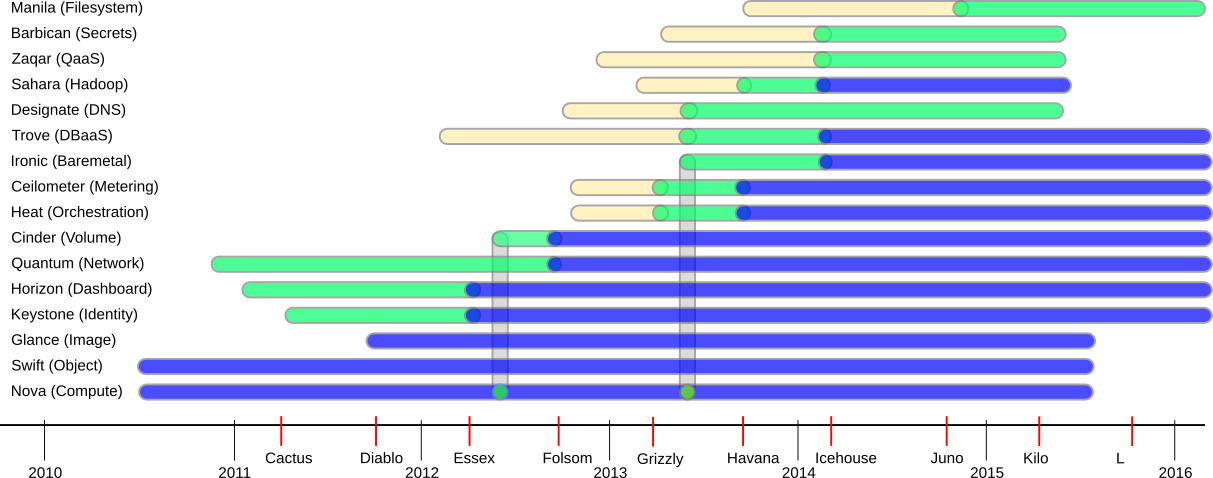
\includegraphics[width=\textwidth]{OpenStack_Components.png}
    \end{center}
\end{frame}

\begin{frame}
    \frametitle{Tempest Tests per Project}
    \begin{center}
        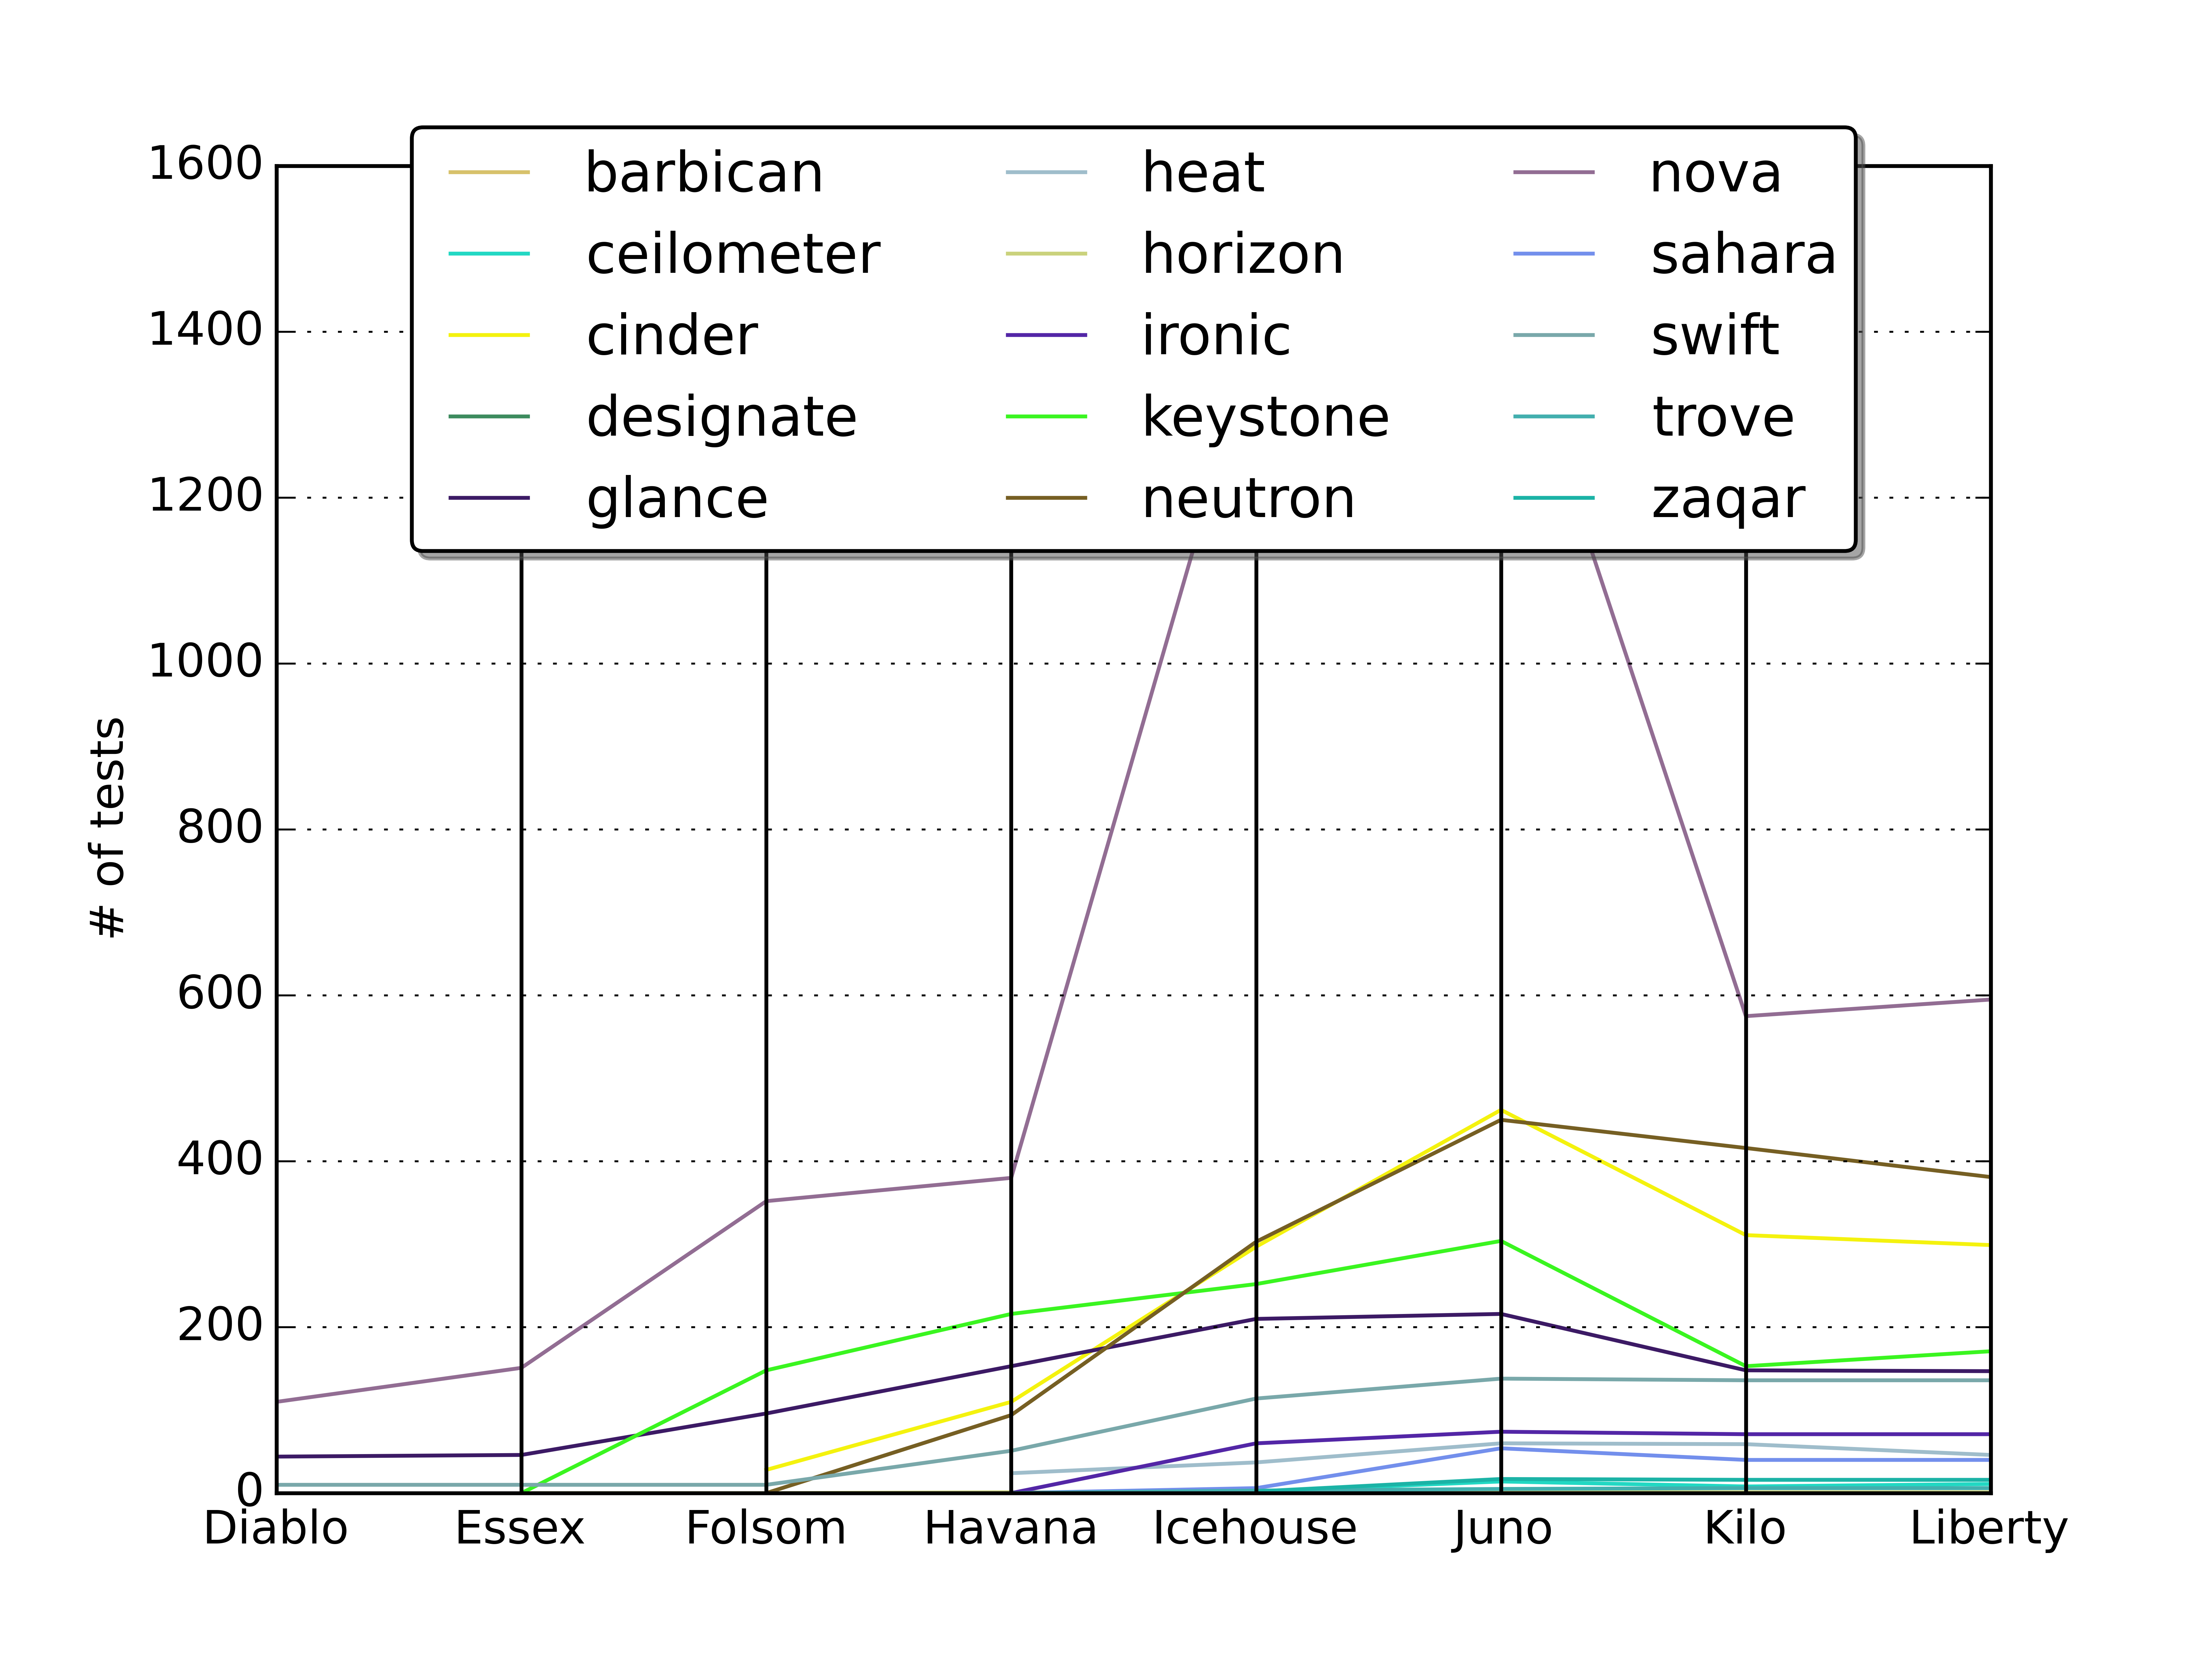
\includegraphics[width=.8\textwidth]{tests_per_proj.png}
    \end{center}
\end{frame}

\begin{frame}
    \frametitle{The Big Tent\ldots}
    \begin{center}
        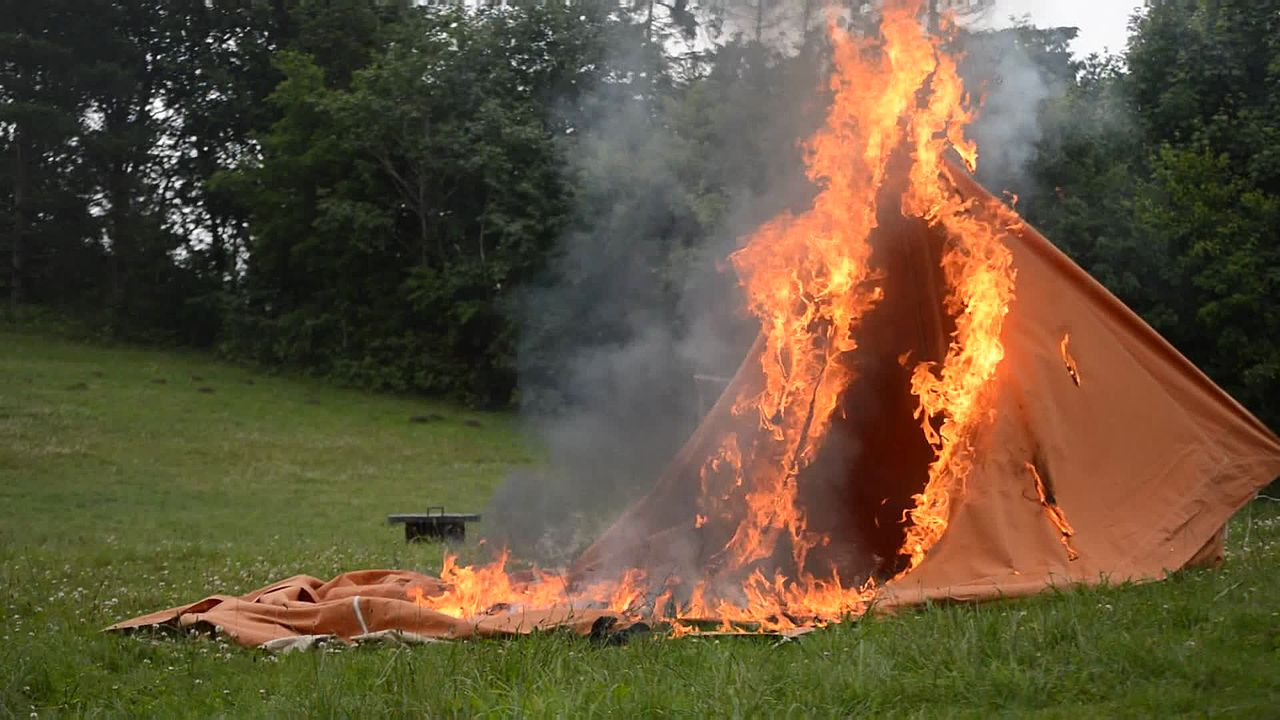
\includegraphics[width=.9\textwidth]{Burning_Tent.jpg}
    \end{center}
\end{frame}

\begin{frame}
    \frametitle{QA in the Big Tent}
    \begin{itemize}
        \item QA projects now directly support base
        \item Provide stable plugin interfaces to expand functionality
        \item Better fits with the growth in projects
    \end{itemize}
\end{frame}

\begin{frame}
    \frametitle{Current Projects QA directly supports in-tree}
    \begin{itemize}
        \item Keystone
        \item Nova
        \item Glance
        \item Cinder
        \item Neutron
        \item Swift
    \end{itemize}
\end{frame}

\section{Current Plugin Interfaces}
\subsection{Devstack Plugins}
\begin{frame}
	\frametitle{Devstack Plugins}
    \begin{itemize}
    \item{Bits of bash code that live outside of devstack tree}
    \item{Called via a strong contract}
    \item{Maintained by the project owners}
    \item{Tested via OpenStack CI}
    \end{itemize}

    \begin{itemize}
    \item{Project plugins}
    	\begin{itemize}
    		\item Installs new OpenStack service as part of devstack
    	\end{itemize}
    \item{Driver / configuration plugins}
    	\begin{itemize}
    		\item Configures existing OpenStack service to use a different driver / backend
    	\end{itemize}
    \item Registry of plugins maintained by the community: \hfill
    \\ http://docs.openstack.org/developer/devstack/plugin-registry.html
    \end{itemize}
\end{frame}

\begin{frame}
    \frametitle{Projects using Devstack Plugins}
    \begin{figure}[p]
    	\centering
    	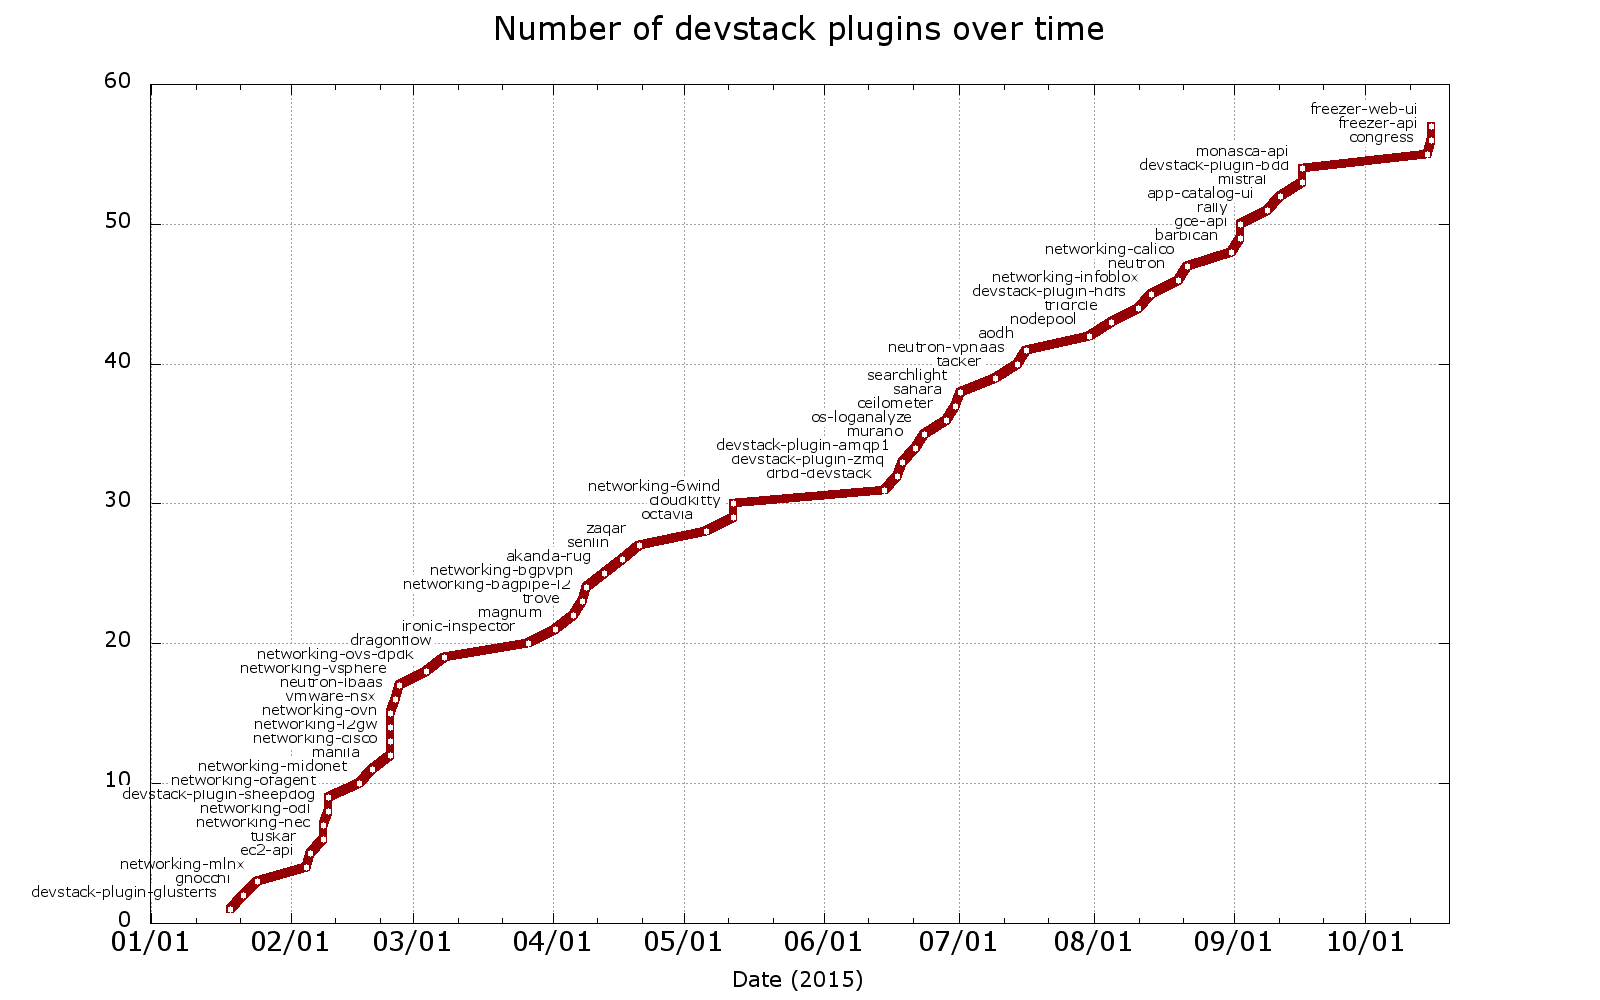
\includegraphics[width=0.8\textwidth]{devstack-plugins.png}
    	\caption{Source: git log --diff-filter=A --format=\%cd --date=short -1 -- devstack/plugin.sh}
    \end{figure}
\end{frame}

\begin{frame}
    \frametitle{Howto write a Devstack Plugin}
\end{frame}

\subsection{Tempest Plugins}
\begin{frame}
    \frametitle{Tempest Plugins}
    \begin{itemize}
        \item Integrates any external tests into a tempest run
        \item Unifies configuration between plugin(s) and in-tree
        \item 
    \end{itemize}
    \begin{itemize}
    	\item{Based on stevedore plugin model}
    	\item{Automatically discovered when installed}
    	\item{Test code built on top of tempest-lib}
    \end{itemize}
\end{frame}

\begin{frame}
    \frametitle{Projects using tempest plugins}
    \begin{figure}[p]
    	\centering
    	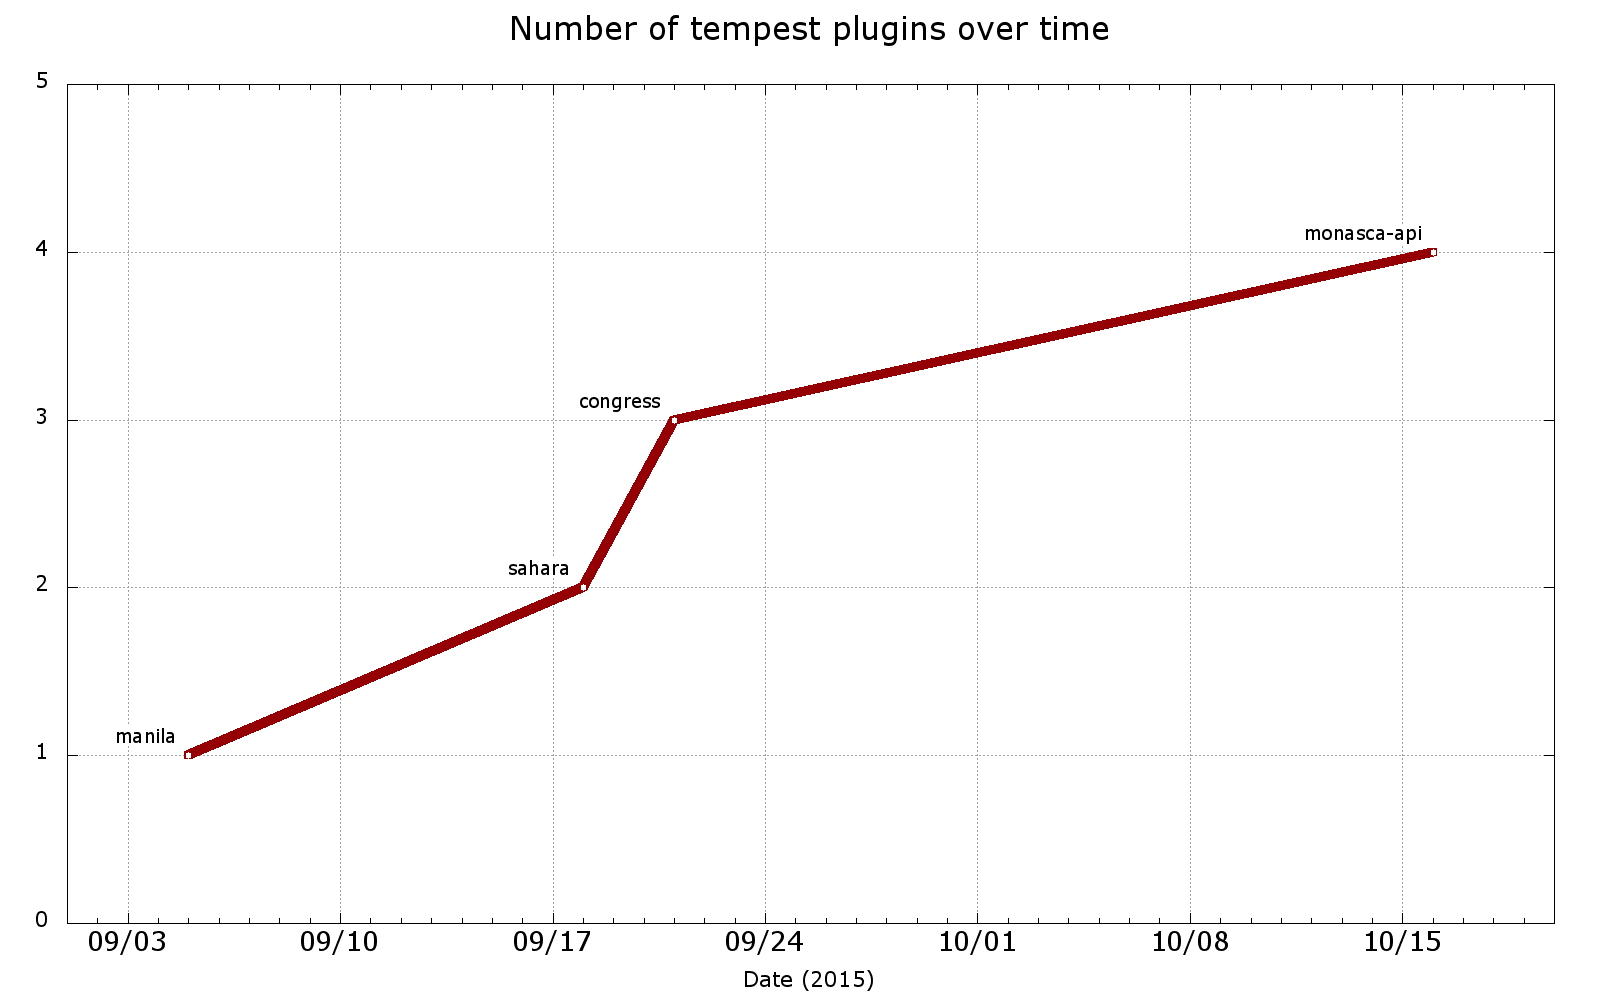
\includegraphics[width=0.8\textwidth]{tempest-plugins.png}
        \caption{Source: git blame -L '/\^{}tempest/,+1' setup.cfg | awk '\{print \$1\}' | xargs git log -1 --format=\%cd --date=short}
    \end{figure}
\end{frame}

\begin{frame}
    \frametitle{Howto Write a Tempest Plugin}
    \begin{itemize}
    	\item{Code can be hosted in existing or dedicated git project}
    	\item{Extend plugins.TempestPlugin from tempest (or tempest-lib)}
    	\item{Implement all abstract methods}
    		\begin{itemize}
    			\item{Test discovery: }
    			\item{Configuration options: }
    		\end{itemize}
    	\item{Check if everything you need is tempest lib}
    	\item{Setup CI to test with your plugin, and keep it tested}
    \end{itemize}
\end{frame}

\subsection{Grenade Plugins}
\begin{frame}
    \frametitle{Grenade Plugins}
\end{frame}

\begin{frame}
	\frametitle{Projects using Grenade Plugins}
    \begin{figure}[p]
    	\centering
    	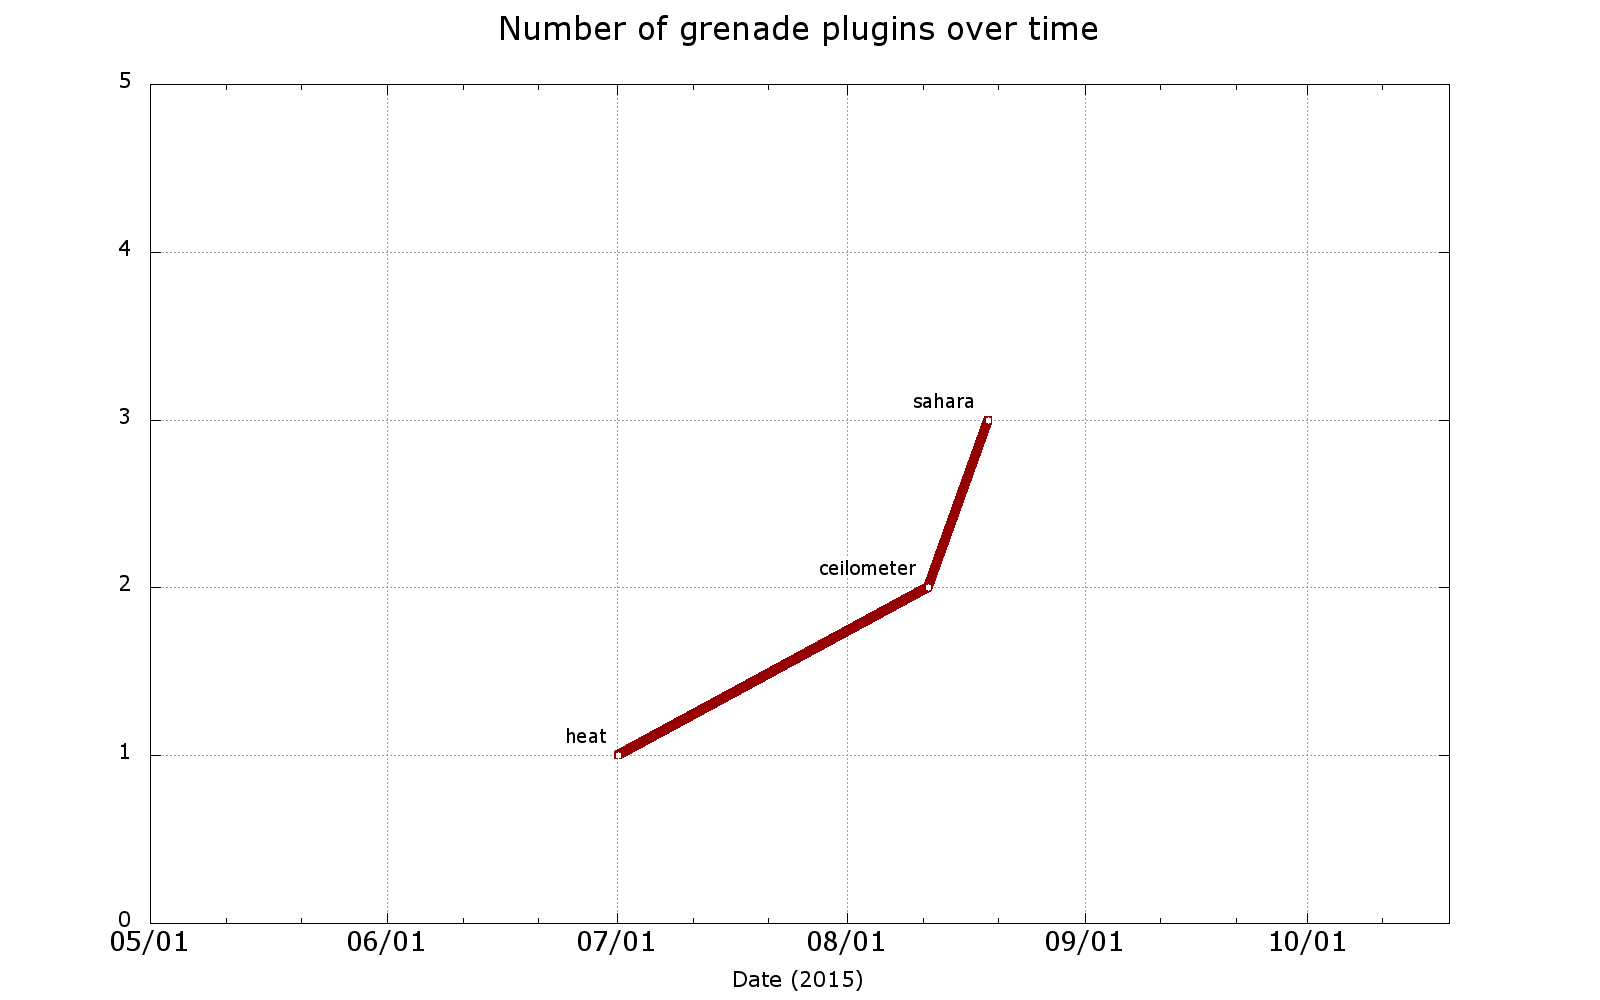
\includegraphics[width=0.8\textwidth]{grenade-plugins.png}
    	\caption{Source: git log --diff-filter=A --format=\%cd --date=short -1 -- devstack/upgrade/upgrade.sh}
    \end{figure}
\end{frame}

\begin{frame}
    \frametitle{Howto Write a Grenade Plugin}
\end{frame}

\section{More Information}
\begin{frame}
\frametitle{Where to get more information}
    \begin{itemize}
        \item Tempest Plugin Docs: \href{http://docs.openstack.org/developer/tempest/plugin.html}{http://docs.openstack.org/developer/tempest/plugin.html}
        \item Devstack Plugin Docs: \href{http://docs.openstack.org/developer/devstack/plugins.html}{http://docs.openstack.org/developer/devstack/plugins.html}
        \item Grenade Plugin Docs: \href{http://docs.openstack.org/developer/grenade/plugins.html}{http://docs.openstack.org/developer/grenade/plugins.html}
        \item openstack-dev ML: \href{mailto:openstack-dev@lists.openstack.org}{openstack-dev@lists.openstack.org}
        \item \#openstack-qa on Freenode
    \end{itemize}
\end{frame}

\section{Questions}
\begin{frame}
\frametitle{Questions?}
\end{frame}

%\section{Extra Info}
\end{document}
